\documentclass{article}
\usepackage{siunitx}
\usepackage{float}

% Language setting
\usepackage[english]{babel}

% Set page size and margins
% Replace `letterpaper' with `a4paper' for UK/EU standard size
\usepackage[letterpaper,top=2cm,bottom=2cm,left=3cm,right=3cm,marginparwidth=1.75cm]{geometry}

% Useful packages
\usepackage{amsmath}
\usepackage{graphicx}
\usepackage[colorlinks=true, allcolors=blue]{hyperref}
\usepackage{algorithm2e}
\RestyleAlgo{ruled}
\title{Efficiency analysis of various Vertex Cover Algorithms}
\begin{document}
\begin{titlepage}
    \begin{center}
        \vspace*{0.5cm}
        \Huge
        \textbf{Efficiency analysis of various Vertex Cover Algorithms }
            
        \vspace{1cm}
        \LARGE
        \bf ECE 650: Final Project     
        \vspace{4.5cm}
         

        \includegraphics[width=0.5\textwidth]{university}
        \vfill
        \textbf{Submitted By:\\
        Abhi Zanzarukiya - 20892635 \\
        Heli Mistry - 20985952}
        \vspace{0.8cm}
            
        \Large
        Electrical and Computer Engineering\\
        University of Waterloo\\
    \end{center}
\end{titlepage}
\begin{abstract}
It is a typical NP-hard optimization problem in computer science to determine a minimum vertex cover. As a result, we have no polynomial time algorithm for solving this problem, and we use approximation algorithms to solve it. This project report shows an analysis of three different approaches to solve the Vertex Cover problem viz.(1)CNF-SAT-VC (2)APPROX-VC-1 (3)APPROX-VC-2. Here we analyze the efficiency of the algorithms by considering a comparison of their running times and approximation ratios. Looking at the results, we observed that CNF-SAT-VC produces the optimal solution, but comparatively has the largest runtime. APPROX-VC-2 has the shortest runtime but does not provide a minimum vertex coverage, whereas APPROX-VC-1 is the most feasible in terms of accuracy and efficiency, despite a slight deviation from providing an optimal solution.
\end{abstract}

\section{Overview}

This project aims to solve the problem of optimal installation of security cameras at traffic intersections to help the police department. We map this optimization problem to the Vertex Cover problem and present three different possible solutions with their analysis.

\section{Definitions}

\subsection{Vertex Cover}

A vertex cover of a graph G= \textsc(V, E) is a subset of vertices $C \subseteq $V, such that each edge $e \in $E is incident to at least one vertex in C. In other words, the vertex cover is a set of vertices that completely covers all edges of a given graph. 

\subsection{MiniSAT}

SAT solvers are tools that are used to check and evaluate the satisfiability of Boolean Satisfiability problems. This evaluated satisfying assignment from the SAT solver is the solution to an NP-complete problem which is represented as a Boolean logic formula. \\

MiniSAT is a minimalistic SAT solver that we have used in our project. This tool is highly modifiable, and through variable and clause elimination it is very efficient.

\subsection{CNF-SAT}

The CNF Satisfiability Problem (CNF-SAT) is a version of the classic combinatorial Satisfiability Problem - Boolean Satisfiability, where the propositional logic is specified in the Conjunctive Normal Form (CNF). In this representation, a given formula of variables is written as a conjunction of clauses. Each clause is a disjunction of literals, and a literal is a variable or its negation.\\

We reduce the vertex cover problem for graph G, to CNF-SAT formula F with four reductions, in polynomial time. This formula F is provided as an input to the SAT-solver MiniSAT. If F is satisfiable, then the satisfiability assignment from the MiniSAT will be our minimum vertex cover.

\subsection{APPROX-VC-1}

This estimated solution to the given problem aims at finding the vertex cover by picking up a vertex with the highest degree in each run and eliminates all its adjacent edges. The process is repeated until all the edges are covered. \\

\begin{algorithm}[H]
\caption{APPROX-VC-1(G)}\label{alg:one}
$C\gets \Phi$\;
\While{$E \neq \Phi $}{
    Find vertex v from V with highest number of incident edges\;
    $C \gets C \cup \{v\}$\;
}
\end{algorithm}


\subsection{APPROX-VC-2}

This is a greedy algorithms where we pick an arbitrary edge, and insert both its endpoints in the vertex cover. Then, we throw away all the attached to these two endpoints and keep going till no uncovered edges are left. \\

\begin{algorithm}[H]
\caption{APPROX-VC-2(G)}\label{alg:two}
$C\gets \Phi$\;
\While{$E \neq \Phi $}{
    Pick an edge $\{u,v\} \in E$\;
    $C \gets C \cup \{u,v\}$\;
    Delete all edges incident to either u or v\;
}
\end{algorithm}

\subsection{Efficiency Metrics}
As part of this experiment, the efficiency of all three algorithms are evaluated by using two quantitative metrics namely Mean Running Time and Approximate Ratio. The details of both metrics are below:

\subsubsection{Mean Running Time}
It is the average time of multiple runs of each algorithm which represents the total time taken by that algorithm to solve a problem. In our case all three algorithms, APPROX-VC-1, APPROX-VC-2 and CNF-SAT-VC are run over multiple inputs of a graph of fixed size of vertex and the time taken is collected and averaged.

\subsubsection{Approximate Ratio}
The approximate ratio here is defined as the ratio of cardinality of vertex cover by  approximate algorithms (APPROX-VC-1 and APPROX-VC-2) to the cardinality of vertex cover by optimal (minimum-size) algorithm CNF-SAT-VC.

\section{Implementation details}

The concept of multithreading is used for this experiment in order to run algorithms concurrently. In total four threads are used to perform the analysis. One thread is used for IO operations like reading the input and parsing the input and then calling the other three threads to run the respective algorithm. Other three threads run respective algorithms over the parsed input and generate results. The required methods for dealing with threads are available in the pthread and time library in C++ which are used here. Methods like \texttt{pthread\_getcpuclockid()} and \texttt{clock\_gettime()} are used to get the clock id of the cpu assigned to the thread and extract the instance of time from that clock respectively.\\

Input data of random instances of graph structure are generated by the \boldsymbol{graphGen}, a random generator for generating graphs of various different vertex sizes \boldsymbol{$$|V|$$}. Here for this experiment we selected 23 different sizes of vertex \boldsymbol{$$|V|$$} ranging from {[2, 17]} in increments of 1 and {[20, 50]} with increments of 5.  Now for each vertex size \boldsymbol{$$|V|$$}, we generate 10 graphs of that size using \boldsymbol{graphGen}. Each such graph is run 10 times against all three algorithms. This results in a total 100 runs of 10 graphs for a given size vertex input. \\

The output data generated by these runs is of the order {(100 x 6)}, where row value 100 represents the output from one run and 6 columns represents different metrics in form of tuple\\

\textit{(ART(SAT-CNF-VC), ART(Approx-VC-1),ART(Approx-VC-2), \nobreak VCSize(Approx-VC-1), VCSize(Approx-VC-2), VCSize(SAT-CNF-VC))}  \\


\textit{where RT{(A)} is running time of Algorithm A in microseconds and VCSize{(A)} is the vertex cover size of Algorithm A.}\\

After generating these results, the average and standard deviation of running time for all three algorithms and the same of approximate ratio for both Approximation algorithms is calculated and used as part of analysis.

\section{Results and Analysis}

\begin{figure}[H]
\centering
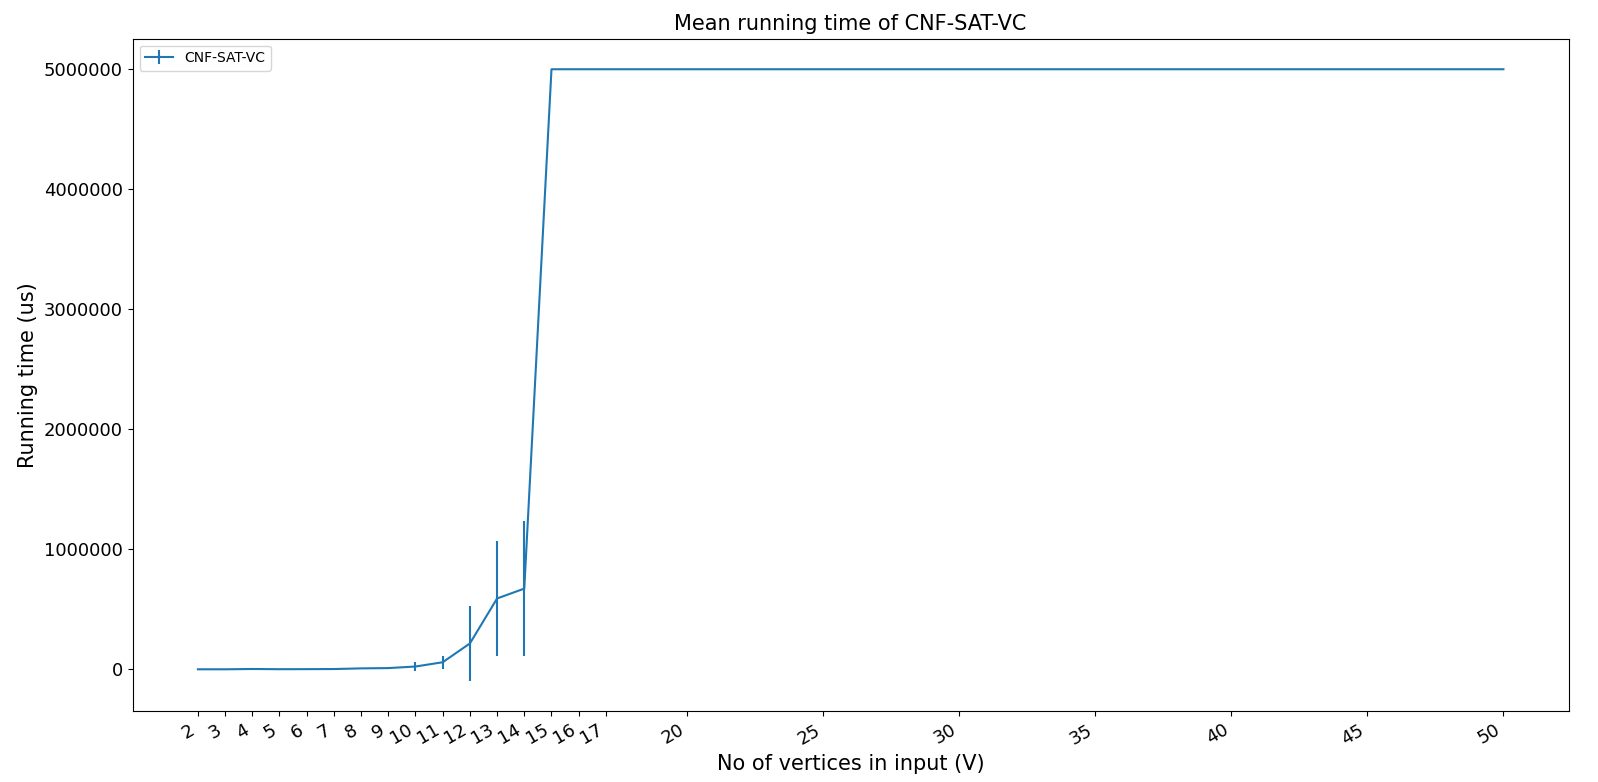
\includegraphics[width=1\textwidth]{Figure1.png}
\caption{\label{fig:Figure1}Mean Running Time plot for all input vertices of CNF-SAT-VC algorithm thread.}
\end{figure}


The average running time of CNF-SAT-VC algorithm is shown in Figure 1 which contains all the values of vertex used as part of analysis. It can be seen from Figure 1 that with the increase in the number of vertices, the time taken by CNF-SAT-VC to generate the solution increases exponentially. The time taken by graphs with vertices  $\boldsymbol{$$|V|$$} \geq $15 is so high that inorder to have the feasibility of the experiment, the timeout of 5 seconds is associated with the CNF-SAT-VC thread. As a result, a flat line ranging for input from {[15, 50]} is seen to be clipped at 5 seconds because of timeout. In order to have the proper resolution of exponential behavior for runtime of this algorithm Figure 2 is plotted with the range of vertices [2,14] where the algorithm is successful in finding a solution before timeout.  \\

\begin{figure}[H]
\centering
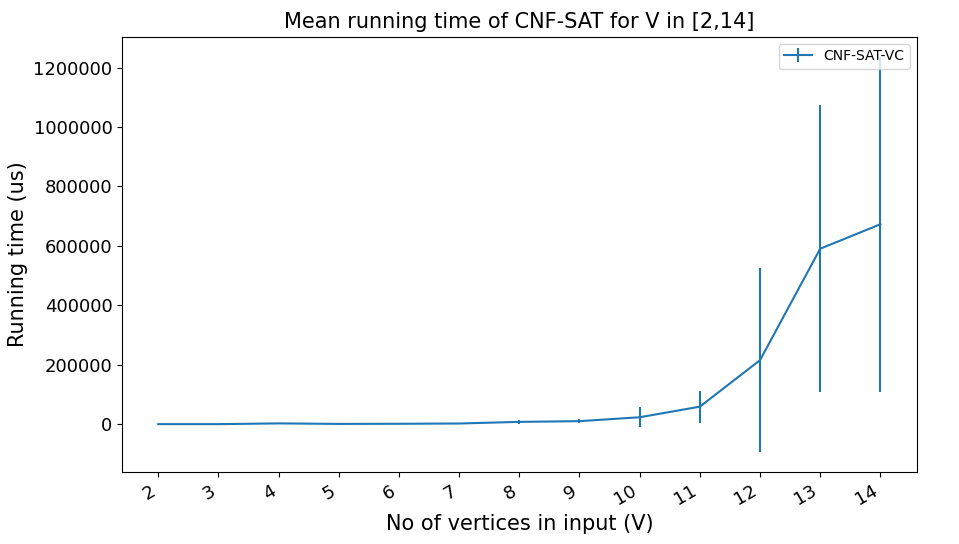
\includegraphics[width=1\textwidth]{Figure2.png}
\caption{\label{fig:figure2}Mean Running Time plot for vertices in range [2,14] of CNF-SAT-VC algorithm thread.}
\end{figure}

The reason for the exponential rise in time can be justified by looking at the formula stating number of clauses and literals involved in reduction from VC to CNF-SAT which is given by 

$$Number\space of\space reductions:  k + k * {V \choose 2} + V * {k \choose 2} + |E|    $$
$$Number of literals : V * k$$
\\
\textit{where  V is the input vertex size, k is the vertex vover size and $|E|$ is the number of edges.  }\\


As V increases the literals and the clauses generated by reduction also increase exponentially. This in turn makes the propositional logic formula F also large. SAT solver (here Minisat) needs a lot of time to generate a satisfiability assignment for such a formula in order to solve the problem. \\

Figure 3 shows the average running time of both approximate algorithms, APPROX-VC-1 and APPROX-VC-2 against all input vertices. It is very clear that the runtime of both these algorithms is comparatively very less compared to that of CNF-SAT-VC algorithm. Till input in range [2,9] the average runtime is almost equal for both algorithms. However, from $\boldsymbol{$$|V|$$} \geq $10, the graph shows divergence and hence it can be observed that APPROX-VC-2 takes less time compared to Approx-VC-1 in this range. The difference in running time is because, APPROX-VC-1 visits the edge list to find the highest degree vertex in order to include it in the vertex cover list. After that the list is traversed to remove edges having that highest degree vertex. Whereas in APPROX-VC-2 the vertices associated with the first edge in edge list is added to list and then the list is traversed to remove edges having these vertices. So, APPROX-VC-1 makes extra iteration over the edge list which increases the time for computing the solution. 

\begin{figure}[H]
\centering
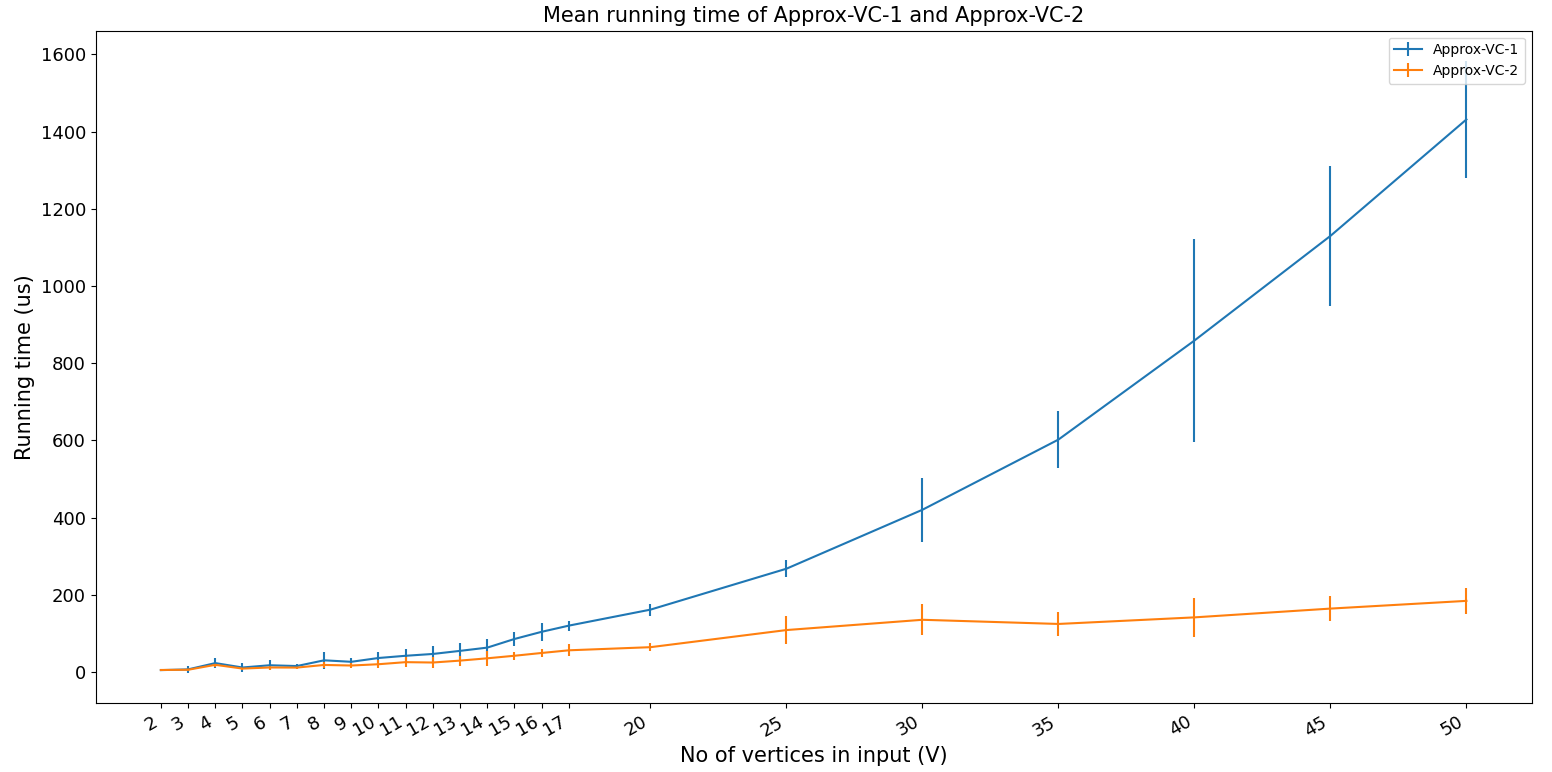
\includegraphics[width=1\textwidth]{Figure3.png}
\caption{\label{fig:figure2}Mean Running Time plot for all input vertices of CNF-SAT-VC algorithm thread.}
\end{figure}

The mean approximation ratio for both APPROX-VC-1 and APPROX-VC-2 is plotted in Figure 4. Here the range of input vertices [2,14] is used because for |V|>=15, CNF-SAT-VC timeouts and as a result size of optimal vertex cover is not obtained resulting in no calculation of Approximate Ratio for $\boldsymbol{$$|V|$$} \geq $15 based on the formula used. It is evident from the result that the accuracy in size of vertex cover is more for APPROX-VC-1 than its counterpart APPROX-VC-2. Infact, the output of cardinality of vertex cover for APPROX-VC-1 is almost equal to that of the optimal CNF-SAT-VC algorithm. This can be deduced by looking at Mean Approximate Ratio for APPROX-VC-1 which is almost equal to 1 with every less deviation. The Mean Approximate Ratio for APPROX-VC-2 is around 1.5 which suggests that more vertex cover is produced by APPROX-VC-2 than CNF-SAT-VC. This high value might be because of the random selection (in our case first in edge list) of edges (thus its vertices) as vertex cover. Also random selection of edges in APPROX-VC-2 results in a big errorbar. The APPROX-VC-1 chooses the vertex with the highest degree as vertex cover and hence more number of edges connected with that vertex gets covered. Thus output size is almost same as that of optimal also and also deviation is less which can be seen by small or almost no errorbar for APPROX-VC-2.

\begin{figure}[H]
\centering
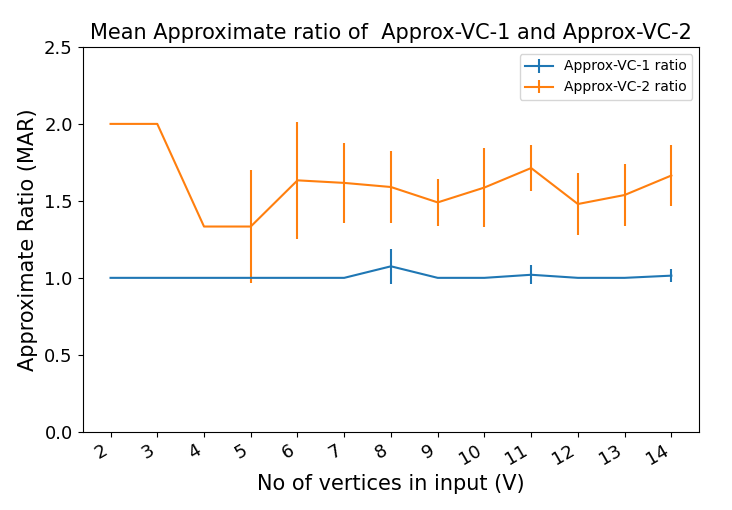
\includegraphics[width=1\textwidth]{Figure4.png}
\caption{\label{fig:figure2}Mean Approximate Ratio for vertices in range [2,14] for Approx-VC-1 and Approx-VC-2.}
\end{figure}



\section{Conclusion}

The CNF-SAT-VC algorithm produces the optimal solution for the minimum-sized vertex cover problem. But, from analysis it's clear that this algorithm's running time increases exponentially with the increase in input vertices and as a result solutions cannot be obtained in a reasonable amount of time for large input graphs. APPROX-AC-V2 runs fastest among all three algorithms but this speed comes at the cost of accuracy as output of APPROX-VC-2 deviates much from the optimal output. If time and accuracy both needs to be considered then APPROX-VC-1 algorithm is the good choice as the output it produces is almost equal to optimal output (vertex cover count). Also, also the algorithm runs in polynomial time and is much faster than optimal algorithm CNF-SAT-VC even for large input graphs.

\end{document}